% --- UNIVERSAL PREAMBLE BLOCK ---
\documentclass[11pt, a4paper]{article}

\usepackage[utf8]{inputenc}
\usepackage[T1]{fontenc}
\usepackage[spanish, es-tabla, es-nodecimaldot]{babel}
\usepackage[a4paper, top=2.5cm, bottom=2.5cm, left=2.5cm, right=2.5cm]{geometry}

\usepackage{graphicx}
% Busca las imagenes en la carpeta img/ o junto al .tex
\graphicspath{{img/}{./}}
\usepackage{float}
\usepackage{hyperref}
\usepackage{enumitem}
\usepackage{xcolor}
\usepackage{listings}
\usepackage{fancyhdr}
\usepackage{tabularx}
\usepackage{longtable}
\usepackage{xltabular}
\usepackage{booktabs}
\usepackage{colortbl}
\usepackage{caption}
\usepackage{amssymb}

\setlist[itemize]{label=-}
\setcounter{secnumdepth}{0}

\definecolor{codegreen}{rgb}{0,0.6,0}
\definecolor{codegray}{rgb}{0.5,0.5,0.5}
\definecolor{codepurple}{rgb}{0.58,0,0.82}
\definecolor{backcolour}{rgb}{0.96,0.96,0.96}

\lstdefinestyle{pythonstyle}{
    backgroundcolor=\color{backcolour},
    commentstyle=\color{codegreen},
    keywordstyle=\color{magenta},
    numberstyle=\tiny\color{codegray},
    stringstyle=\color{codepurple},
    basicstyle=\ttfamily\small,
    breakatwhitespace=false,
    breaklines=true,
    captionpos=b,
    keepspaces=true,
    numbers=left,
    numbersep=5pt,
    showspaces=false,
    showstringspaces=false,
    showtabs=false,
    tabsize=4,
    language=Python,
    extendedchars=true,
    literate={á}{{\'a}}1 {é}{{\'e}}1 {í}{{\'i}}1 {ó}{{\'o}}1 {ú}{{\'u}}1 {ñ}{{\~n}}1 {Á}{{\'A}}1 {É}{{\'E}}1 {Í}{{\'I}}1 {Ó}{{\'O}}1 {Ú}{{\'U}}1 {Ñ}{{\~N}}1 {π}{{$\pi$}}1 {²}{{$^2$}}1 {³}{{$^3$}}1 {¿}{{?`}}1
}
\lstset{style=pythonstyle}

\hypersetup{
    colorlinks=true,
    linkcolor=black,
    filecolor=magenta,
    urlcolor=blue,
    pdftitle={Actividad 4 - POO},
}

% Comando auxiliar para dibujar un cuadro de clase estilo UML
\newcommand{\clasebox}[3]{%
\begin{center}
\begin{tabular}{|l|}
\hline
\textbf{#1} \\
\hline
#2
\hline
#3
\hline
\end{tabular}
\end{center}
}

% Comando auxiliar para dibujar un objeto estilo UML (nombre subrayado)
\newcommand{\objetobox}[2]{%
\begin{center}
\begin{tabular}{|l|}
\hline
\underline{\textbf{#1}} \\
\hline
#2
\hline
\end{tabular}
\end{center}
}

\begin{document}

% ---------------------------------------------------------
% PORTADA
% ---------------------------------------------------------
\begin{titlepage}
    \centering
    \vspace*{1cm}

    {\huge \textbf{Universidad Nacional de Colombia}\par}
    \vspace{0.5cm}
    {\Large Facultad de Minas\par}
    \vspace{1.5cm}

    {\Large \textbf{Programación Orientada a Objetos 2026-2}\par}
    \vspace{2cm}

    {\huge \textbf{Actividad 4}\par}
    \vspace{0.5cm}
    {\large Gestión de excepciones y lectura de archivos con interfaz gráfica: ejercicios 6.4 a 6.8\par}

    \vspace{3cm}

    \textbf{Presentado por:}\par
    \vspace{0.5cm}
    {\Large \textbf{Natalia Patricia Remolina Rodríguez}\par}

    \vspace{2cm}

    \textbf{Docente:}\par
    Walter Hugo Arboleda Mazo\par

    \vspace{2cm}

    Medellín, Colombia\par
    17 de noviembre de 2026
\end{titlepage}

% ---------------------------------------------------------
% EJERCICIO 4.1
% ---------------------------------------------------------
\section{Ejercicio 6.4. Excepciones: clase PruebaExcepciones}

\subsection{Enunciado}
Se plantea un programa con dos bloques \texttt{try} que generan excepciones y deben ser
gestionadas, y se pregunta cuál es el resultado de su ejecución, es decir, qué se imprime en
pantalla y en qué orden. La solución lleva ese programa a una interfaz gráfica, de modo que la
salida se vea en la ventana en lugar de la consola.

\medskip
\noindent El primer bloque provoca una división por cero, que se captura como excepción
aritmética. El segundo usa un objeto nulo, que no corresponde a una excepción aritmética sino a
una general. En ambos casos el bloque \texttt{finally} se ejecuta siempre. El resultado es:

\begin{itemize}
    \item Ingresando al primer try
    \item División por cero
    \item Ingresando al primer finally
    \item Ingresando al segundo try
    \item Ocurrió una excepción
    \item Ingresando al segundo finally
\end{itemize}

\noindent \textbf{Enlace al repositorio en GitHub:} \\
\url{https://github.com/NatoRemolina/UNAL-Programacion-Orientada-a-Objetos/blob/main/actividad-04/ejercicio1.py}

\subsection{Diagrama de clases}
\clasebox{PruebaExcepciones}
{%
- mensajes \\
}
{%
+ ejecutar() \\
}

\clasebox{VentanaPrueba}
{%
- color\_fondo \\
- color\_texto \\
- txt\_salida \\
}
{%
+ \_crear\_componentes() \\
+ action\_ejecutar() \\
+ action\_limpiar() \\
}

\noindent \textbf{Relaciones:}
\begin{itemize}
    \item \texttt{VentanaPrueba} hereda de \texttt{tk.Tk}: es la ventana principal de la aplicación.
    \item \texttt{VentanaPrueba} usa a \texttt{PruebaExcepciones} (dependencia): le pide la lista de mensajes y los escribe en pantalla, de manera que la lógica queda separada de la presentación.
\end{itemize}

\subsection{Casos de uso}
\begin{table}[H]
\centering
\begin{tabularx}{\textwidth}{@{}l X@{}}
\toprule
\textbf{Caso de uso} & CU-01: Ejecutar el programa \\
\midrule
\textbf{Actor} & Usuario \\
\textbf{Precondición} & La ventana está abierta. \\
\textbf{Flujo principal} & 1. El usuario presiona el botón \textit{Ejecutar}. \newline 2. El sistema recorre los dos bloques \texttt{try}. \newline 3. El sistema captura cada excepción y registra el mensaje correspondiente. \newline 4. El sistema ejecuta los dos bloques \texttt{finally}. \newline 5. El sistema muestra los seis mensajes en el orden en que se produjeron. \\
\textbf{Postcondición} & La salida del programa queda visible en la ventana. \\
\bottomrule
\end{tabularx}
\end{table}

\begin{table}[H]
\centering
\begin{tabularx}{\textwidth}{@{}l X@{}}
\toprule
\textbf{Caso de uso} & CU-02: Limpiar la salida \\
\midrule
\textbf{Actor} & Usuario \\
\textbf{Precondición} & La ventana está abierta. \\
\textbf{Flujo principal} & 1. El usuario presiona el botón \textit{Limpiar}. \newline 2. El sistema borra el contenido del área de salida. \\
\textbf{Postcondición} & La ventana queda en su estado inicial. \\
\bottomrule
\end{tabularx}
\end{table}

\subsection{Interfaz de usuario}
\begin{figure}[H]
    \centering
    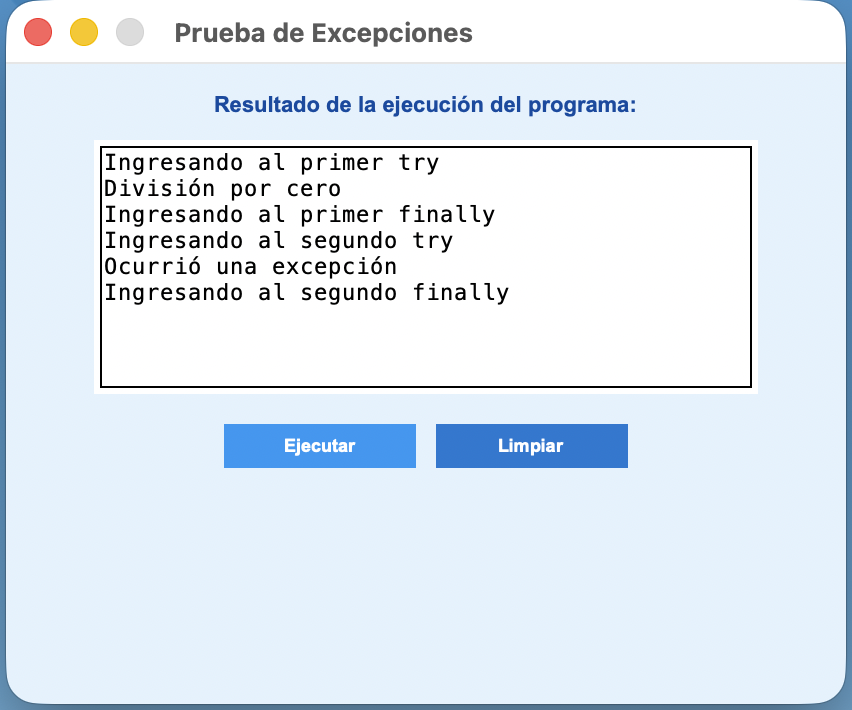
\includegraphics[width=0.62\textwidth]{excepciones.png}
    \caption{Salida del programa tras presionar el botón Ejecutar.}
\end{figure}

\subsection{Código fuente}
\begin{lstlisting}
import tkinter as tk
from tkinter import ttk

# ==========================================
# CLASE LÓGICA (Modelo)
# ==========================================
class PruebaExcepciones:
    """Reproduce los dos bloques try del ejercicio y guarda, en orden,
    los mensajes que el programa va imprimiendo."""

    def __init__(self):
        self.mensajes = []

    def ejecutar(self):
        self.mensajes = []

        # Primer bloque try: se provoca una división por cero
        try:
            self.mensajes.append("Ingresando al primer try")
            cociente = 10000 / 0
            # Esta instrucción nunca se ejecuta
            self.mensajes.append("Después de la división")
        except ZeroDivisionError:
            self.mensajes.append("División por cero")
        finally:
            # El bloque finally siempre se ejecuta, ocurra o no la excepción
            self.mensajes.append("Ingresando al primer finally")

        # Segundo bloque try: se usa un objeto nulo
        try:
            self.mensajes.append("Ingresando al segundo try")
            objeto = None
            objeto.upper()
            # Esta instrucción nunca se ejecuta
            self.mensajes.append("Imprimiendo objeto")
        except ZeroDivisionError:
            # La excepción lanzada no es de este tipo, así que no entra aquí
            self.mensajes.append("División por cero")
        except Exception:
            self.mensajes.append("Ocurrió una excepción")
        finally:
            self.mensajes.append("Ingresando al segundo finally")

        return self.mensajes

# ==========================================
# CLASE INTERFAZ GRÁFICA (Vista/Controlador)
# ==========================================
class VentanaPrueba(tk.Tk):
    """Ventana que ejecuta el programa y muestra su salida en pantalla."""

    def __init__(self):
        super().__init__()

        # Paleta de colores azul
        self.color_fondo = "#e3f2fd"
        self.color_texto = "#0d47a1"

        self.title("Prueba de Excepciones")
        self.geometry("420x320")
        self.resizable(False, False)
        self.configure(bg=self.color_fondo)

        self._crear_componentes()
        self.eval('tk::PlaceWindow . center')

    def _crear_componentes(self):
        tk.Label(self, text="Resultado de la ejecución del programa:",
                 bg=self.color_fondo, fg=self.color_texto,
                 font=("Arial", 11, "bold")).pack(pady=10)

        # Área donde se muestran los mensajes, en el orden en que se imprimen
        self.txt_salida = tk.Text(self, height=9, width=46, bd=1, relief="solid")
        self.txt_salida.pack(padx=20)
        self.txt_salida.config(state="disabled")

        # Botones con estilo azul.
        # Se usa ttk con el tema "clam" porque los botones tk no admiten
        # colores de fondo en macOS y quedarían ilegibles.
        estilo = ttk.Style(self)
        estilo.theme_use("clam")
        estilo.configure("Ejecutar.TButton", background="#2196f3", foreground="white",
                         font=("Arial", 9, "bold"), borderwidth=0, focuscolor="#2196f3")
        estilo.map("Ejecutar.TButton", background=[("active", "#1565c0")])
        estilo.configure("Limpiar.TButton", background="#1976d2", foreground="white",
                         font=("Arial", 9, "bold"), borderwidth=0, focuscolor="#1976d2")
        estilo.map("Limpiar.TButton", background=[("active", "#0d47a1")])

        marco = tk.Frame(self, bg=self.color_fondo)
        marco.pack(pady=15)
        ttk.Button(marco, text="Ejecutar", command=self.action_ejecutar,
                   style="Ejecutar.TButton", width=14).pack(side="left", padx=5)
        ttk.Button(marco, text="Limpiar", command=self.action_limpiar,
                   style="Limpiar.TButton", width=14).pack(side="left", padx=5)

    def action_ejecutar(self):
        """Ejecuta el programa y escribe sus mensajes en la ventana."""
        prueba = PruebaExcepciones()
        mensajes = prueba.ejecutar()

        self.txt_salida.config(state="normal")
        self.txt_salida.delete("1.0", tk.END)
        for mensaje in mensajes:
            self.txt_salida.insert(tk.END, mensaje + "\n")
        self.txt_salida.config(state="disabled")

    def action_limpiar(self):
        """Deja la ventana en su estado inicial."""
        self.txt_salida.config(state="normal")
        self.txt_salida.delete("1.0", tk.END)
        self.txt_salida.config(state="disabled")

# ==========================================
# BLOQUE PRINCIPAL
# ==========================================
if __name__ == "__main__":
    app = VentanaPrueba()
    app.mainloop()
\end{lstlisting}

\newpage
% ---------------------------------------------------------
% EJERCICIO 4.2
% ---------------------------------------------------------
\section{Ejercicio 6.5. Lanzamiento de excepciones: clase Vendedor}

\subsection{Enunciado}
Se requiere implementar una clase \texttt{Vendedor} con los atributos nombre, apellidos y
edad, y un constructor que los inicialice. La clase posee un método para imprimir sus atributos
y un método para verificar la edad:

\begin{itemize}
    \item Si el vendedor no es mayor de 18 años se lanza una excepción con el mensaje
          \textit{``El vendedor debe ser mayor de 18 años''}.
    \item Si la edad no está en el rango de 0 a 120 se lanza una excepción con el mensaje
          \textit{``La edad no puede ser negativa ni mayor a 120''}.
    \item Solo si la edad cumple ambos requisitos se puede instanciar el objeto.
\end{itemize}

\noindent Los datos del vendedor se ingresan desde la ventana.

\noindent \textbf{Enlace al repositorio en GitHub:} \\
\url{https://github.com/NatoRemolina/UNAL-Programacion-Orientada-a-Objetos/blob/main/actividad-04/ejercicio2.py}

\subsection{Diagrama de clases}
\clasebox{Vendedor}
{%
- nombre \\
- apellidos \\
- edad \\
}
{%
+ verificar\_edad() \\
+ imprimir() \\
}

\clasebox{VentanaVendedor}
{%
- color\_fondo \\
- color\_texto \\
- entradas \\
- lbl\_resultado \\
}
{%
+ \_crear\_componentes() \\
+ action\_registrar() \\
+ action\_limpiar() \\
}

\noindent \textbf{Relaciones:}
\begin{itemize}
    \item \texttt{VentanaVendedor} hereda de \texttt{tk.Tk}.
    \item \texttt{VentanaVendedor} usa a \texttt{Vendedor} (dependencia): intenta construir el objeto y captura la excepción que este lanza cuando la edad no es válida.
\end{itemize}

\subsection{Casos de uso}
\begin{table}[H]
\centering
\begin{tabularx}{\textwidth}{@{}l X@{}}
\toprule
\textbf{Caso de uso} & CU-01: Registrar un vendedor \\
\midrule
\textbf{Actor} & Usuario \\
\textbf{Precondición} & La ventana está abierta. \\
\textbf{Flujo principal} & 1. El usuario ingresa nombre, apellidos y edad. \newline 2. El usuario presiona el botón \textit{Registrar}. \newline 3. El sistema verifica que los tres campos estén diligenciados. \newline 4. El sistema convierte la edad a número entero. \newline 5. El sistema crea el objeto \texttt{Vendedor}, que verifica la edad. \newline 6. El sistema muestra los datos del vendedor registrado. \\
\textbf{Flujo alterno A} & En el paso 3, si falta algún campo, el sistema muestra la alerta \textit{``Debe diligenciar los tres campos''}. El caso de uso termina. \\
\textbf{Flujo alterno B} & En el paso 4, si la edad no es un número entero, el sistema muestra la alerta \textit{``La edad debe ser un número entero''}. El caso de uso termina. \\
\textbf{Flujo alterno C} & En el paso 5, si la edad es 18 años o menos, o está fuera del rango de 0 a 120, la clase lanza la excepción y el sistema muestra su mensaje. El objeto no se crea y el caso de uso termina. \\
\textbf{Postcondición} & Los datos del vendedor quedan visibles en la ventana. \\
\bottomrule
\end{tabularx}
\end{table}

\begin{table}[H]
\centering
\begin{tabularx}{\textwidth}{@{}l X@{}}
\toprule
\textbf{Caso de uso} & CU-02: Limpiar el formulario \\
\midrule
\textbf{Actor} & Usuario \\
\textbf{Precondición} & La ventana está abierta. \\
\textbf{Flujo principal} & 1. El usuario presiona el botón \textit{Limpiar}. \newline 2. El sistema borra los tres campos y el resultado. \\
\textbf{Postcondición} & La ventana queda lista para un nuevo registro. \\
\bottomrule
\end{tabularx}
\end{table}

\subsection{Interfaz de usuario}
\begin{figure}[H]
    \centering
    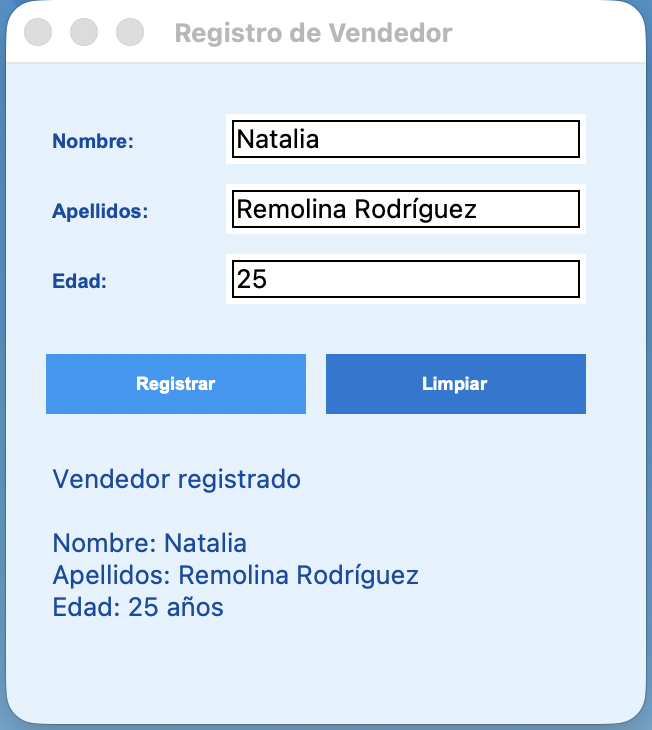
\includegraphics[width=0.46\textwidth]{vendedor.png}
    \caption{Registro exitoso de un vendedor mayor de edad.}
\end{figure}

\subsection{Código fuente}
\begin{lstlisting}
import tkinter as tk
from tkinter import messagebox, ttk

# ==========================================
# CLASE LÓGICA (Modelo)
# ==========================================
class Vendedor:
    """Modela un vendedor y valida su edad antes de crear el objeto."""

    def __init__(self, nombre, apellidos, edad):
        # La edad se verifica primero: si no es válida, el objeto no se crea
        self.verificar_edad(edad)
        self.nombre = nombre
        self.apellidos = apellidos
        self.edad = edad

    def verificar_edad(self, edad):
        """Lanza una excepción si la edad no cumple los requisitos."""
        if edad < 0 or edad > 120:
            raise ValueError("La edad no puede ser negativa ni mayor a 120")
        if edad <= 18:
            raise ValueError("El vendedor debe ser mayor de 18 años")

    def imprimir(self):
        """Retorna los valores de los atributos del vendedor."""
        return (f"Nombre: {self.nombre}\n"
                f"Apellidos: {self.apellidos}\n"
                f"Edad: {self.edad} años")

# ==========================================
# CLASE INTERFAZ GRÁFICA (Vista/Controlador)
# ==========================================
class VentanaVendedor(tk.Tk):
    """Ventana que solicita los datos del vendedor y muestra el resultado."""

    def __init__(self):
        super().__init__()

        # Paleta de colores azul
        self.color_fondo = "#e3f2fd"
        self.color_texto = "#0d47a1"

        self.title("Registro de Vendedor")
        self.geometry("320x330")
        self.resizable(False, False)
        self.configure(bg=self.color_fondo)

        self._crear_componentes()
        self.eval('tk::PlaceWindow . center')

    def _crear_componentes(self):
        etiquetas = ["Nombre:", "Apellidos:", "Edad:"]
        self.entradas = []

        for i, texto in enumerate(etiquetas):
            tk.Label(self, text=texto, anchor="w", bg=self.color_fondo,
                     fg=self.color_texto, font=("Arial", 10, "bold")
                     ).place(x=20, y=25 + (i * 35), width=80, height=25)

            txt_entry = tk.Entry(self, bd=1, relief="solid")
            txt_entry.place(x=110, y=25 + (i * 35), width=180, height=25)
            self.entradas.append(txt_entry)

        # Botones con estilo azul.
        # Se usa ttk con el tema "clam" porque los botones tk no admiten
        # colores de fondo en macOS y quedarían ilegibles.
        estilo = ttk.Style(self)
        estilo.theme_use("clam")
        estilo.configure("Registrar.TButton", background="#2196f3", foreground="white",
                         font=("Arial", 9, "bold"), borderwidth=0, focuscolor="#2196f3")
        estilo.map("Registrar.TButton", background=[("active", "#1565c0")])
        estilo.configure("Limpiar.TButton", background="#1976d2", foreground="white",
                         font=("Arial", 9, "bold"), borderwidth=0, focuscolor="#1976d2")
        estilo.map("Limpiar.TButton", background=[("active", "#0d47a1")])

        ttk.Button(self, text="Registrar", command=self.action_registrar,
                   style="Registrar.TButton").place(x=20, y=145, width=130, height=30)
        ttk.Button(self, text="Limpiar", command=self.action_limpiar,
                   style="Limpiar.TButton").place(x=160, y=145, width=130, height=30)

        self.lbl_resultado = tk.Label(self, text="", bg=self.color_fondo,
                                      fg=self.color_texto, justify="left", anchor="nw")
        self.lbl_resultado.place(x=20, y=195, width=270, height=110)

    def action_registrar(self):
        """Crea el vendedor y muestra sus datos, o la excepción generada."""
        nombre, apellidos, edad_texto = [e.get().strip() for e in self.entradas]

        if not nombre or not apellidos or not edad_texto:
            messagebox.showwarning("Datos incompletos",
                                   "Debe diligenciar los tres campos.")
            return

        try:
            # La edad debe ser un número entero
            edad = int(edad_texto)
        except ValueError:
            messagebox.showerror("Error", "La edad debe ser un número entero.")
            return

        try:
            vendedor = Vendedor(nombre, apellidos, edad)
            self.lbl_resultado.config(text="Vendedor registrado\n\n" + vendedor.imprimir())
        except ValueError as excepcion:
            # Se captura la excepción lanzada por verificar_edad
            self.lbl_resultado.config(text="")
            messagebox.showerror("Edad no válida", str(excepcion))

    def action_limpiar(self):
        """Deja la ventana en su estado inicial."""
        for entrada in self.entradas:
            entrada.delete(0, tk.END)
        self.lbl_resultado.config(text="")

# ==========================================
# BLOQUE PRINCIPAL
# ==========================================
if __name__ == "__main__":
    app = VentanaVendedor()
    app.mainloop()
\end{lstlisting}

\newpage
% ---------------------------------------------------------
% EJERCICIO 4.3
% ---------------------------------------------------------
\section{Ejercicio 6.6. Catchs múltiples: clase CálculosNuméricos}

\subsection{Enunciado}
Se requiere definir una clase \texttt{CalculosNumericos} que realice dos operaciones, ambas
con métodos estáticos que reciben un valor decimal como parámetro:

\begin{itemize}
    \item Calcular el logaritmo neperiano. Si el valor no es positivo se genera una excepción
          aritmética.
    \item Calcular la raíz cuadrada. Si el valor no es positivo se genera una excepción
          aritmética.
\end{itemize}

\noindent El valor se ingresa desde la ventana. El programa debe capturar tanto la excepción
aritmética como la que se produce cuando el dato ingresado no es numérico.

\noindent \textbf{Enlace al repositorio en GitHub:} \\
\url{https://github.com/NatoRemolina/UNAL-Programacion-Orientada-a-Objetos/blob/main/actividad-04/ejercicio3.py}

\subsection{Diagrama de clases}
\clasebox{CalculosNumericos}
{%
\textit{(sin atributos propios)} \\
}
{%
+ logaritmo\_neperiano() \\
+ raiz\_cuadrada() \\
}

\clasebox{VentanaCalculos}
{%
- color\_fondo \\
- color\_texto \\
- txt\_valor \\
- lbl\_logaritmo \\
- lbl\_raiz \\
}
{%
+ \_crear\_componentes() \\
+ action\_calcular() \\
+ action\_limpiar() \\
}

\noindent \textbf{Relaciones:}
\begin{itemize}
    \item \texttt{VentanaCalculos} hereda de \texttt{tk.Tk}.
    \item \texttt{logaritmo\_neperiano()} y \texttt{raiz\_cuadrada()} son métodos estáticos: se invocan sobre la clase \texttt{CalculosNumericos} sin necesidad de crear un objeto.
\end{itemize}

\subsection{Casos de uso}
\begin{table}[H]
\centering
\begin{tabularx}{\textwidth}{@{}l X@{}}
\toprule
\textbf{Caso de uso} & CU-01: Calcular el logaritmo y la raíz \\
\midrule
\textbf{Actor} & Usuario \\
\textbf{Precondición} & La ventana está abierta. \\
\textbf{Flujo principal} & 1. El usuario ingresa un valor. \newline 2. El usuario presiona el botón \textit{Calcular}. \newline 3. El sistema convierte el valor a número decimal. \newline 4. El sistema invoca los dos métodos estáticos de la clase. \newline 5. El sistema muestra ambos resultados con cuatro decimales. \\
\textbf{Flujo alterno A} & En el paso 3, si el dato no es numérico, el sistema muestra la alerta \textit{``Debe ingresar un valor numérico''}. El caso de uso termina. \\
\textbf{Flujo alterno B} & En el paso 4, si el valor no es positivo, la clase lanza una excepción aritmética y el sistema muestra su mensaje. No se calcula nada y el caso de uso termina. \\
\textbf{Postcondición} & Los dos resultados quedan visibles en la ventana. \\
\bottomrule
\end{tabularx}
\end{table}

\subsection{Interfaz de usuario}
\begin{figure}[H]
    \centering
    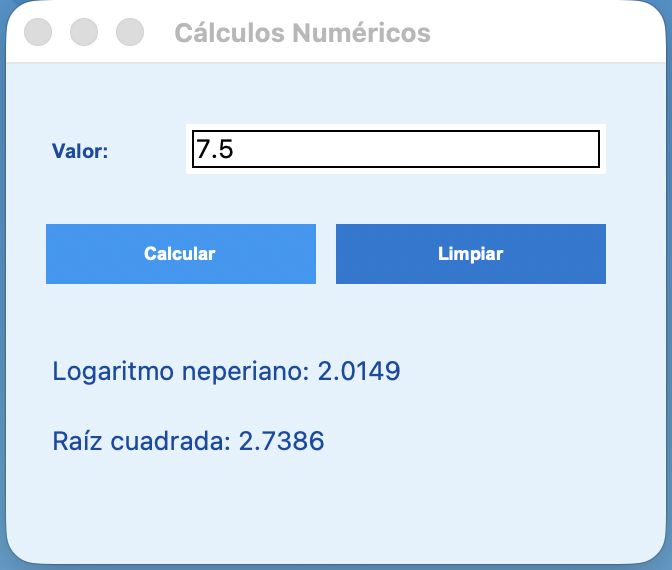
\includegraphics[width=0.48\textwidth]{calculos.png}
    \caption{Cálculo del logaritmo neperiano y la raíz cuadrada de 7.5.}
\end{figure}

\subsection{Código fuente}
\begin{lstlisting}
import tkinter as tk
from tkinter import messagebox, ttk
import math

# ==========================================
# CLASE LÓGICA (Modelo)
# ==========================================
class CalculosNumericos:
    """Realiza dos cálculos matemáticos con métodos estáticos.
    Si el valor recibido no es positivo se genera una excepción aritmética."""

    @staticmethod
    def logaritmo_neperiano(valor):
        if valor <= 0:
            raise ArithmeticError("El logaritmo solo existe para valores positivos")
        return math.log(valor)

    @staticmethod
    def raiz_cuadrada(valor):
        if valor <= 0:
            raise ArithmeticError("La raíz cuadrada solo se calcula para valores positivos")
        return math.sqrt(valor)

# ==========================================
# CLASE INTERFAZ GRÁFICA (Vista/Controlador)
# ==========================================
class VentanaCalculos(tk.Tk):
    """Ventana que solicita un valor y muestra sus dos cálculos."""

    def __init__(self):
        super().__init__()

        # Paleta de colores azul
        self.color_fondo = "#e3f2fd"
        self.color_texto = "#0d47a1"

        self.title("Cálculos Numéricos")
        self.geometry("330x250")
        self.resizable(False, False)
        self.configure(bg=self.color_fondo)

        self._crear_componentes()
        self.eval('tk::PlaceWindow . center')

    def _crear_componentes(self):
        tk.Label(self, text="Valor:", anchor="w", bg=self.color_fondo,
                 fg=self.color_texto, font=("Arial", 10, "bold")
                 ).place(x=20, y=30, width=60, height=25)

        self.txt_valor = tk.Entry(self, bd=1, relief="solid")
        self.txt_valor.place(x=90, y=30, width=210, height=25)

        # Botones con estilo azul.
        # Se usa ttk con el tema "clam" porque los botones tk no admiten
        # colores de fondo en macOS y quedarían ilegibles.
        estilo = ttk.Style(self)
        estilo.theme_use("clam")
        estilo.configure("Calcular.TButton", background="#2196f3", foreground="white",
                         font=("Arial", 9, "bold"), borderwidth=0, focuscolor="#2196f3")
        estilo.map("Calcular.TButton", background=[("active", "#1565c0")])
        estilo.configure("Limpiar.TButton", background="#1976d2", foreground="white",
                         font=("Arial", 9, "bold"), borderwidth=0, focuscolor="#1976d2")
        estilo.map("Limpiar.TButton", background=[("active", "#0d47a1")])

        ttk.Button(self, text="Calcular", command=self.action_calcular,
                   style="Calcular.TButton").place(x=20, y=80, width=135, height=30)
        ttk.Button(self, text="Limpiar", command=self.action_limpiar,
                   style="Limpiar.TButton").place(x=165, y=80, width=135, height=30)

        resultado_style = {"bg": self.color_fondo, "fg": self.color_texto, "anchor": "w"}

        self.lbl_logaritmo = tk.Label(self, text="Logaritmo neperiano: ", **resultado_style)
        self.lbl_logaritmo.place(x=20, y=140, width=280, height=25)

        self.lbl_raiz = tk.Label(self, text="Raíz cuadrada: ", **resultado_style)
        self.lbl_raiz.place(x=20, y=175, width=280, height=25)

    def action_calcular(self):
        """Calcula ambos resultados y gestiona las excepciones posibles."""
        try:
            # Si el texto no es numérico se genera una excepción de conversión
            valor = float(self.txt_valor.get())
        except ValueError:
            messagebox.showerror("Error", "Debe ingresar un valor numérico.")
            return

        try:
            logaritmo = CalculosNumericos.logaritmo_neperiano(valor)
            raiz = CalculosNumericos.raiz_cuadrada(valor)
            self.lbl_logaritmo.config(text=f"Logaritmo neperiano: {logaritmo:.4f}")
            self.lbl_raiz.config(text=f"Raíz cuadrada: {raiz:.4f}")
        except ArithmeticError as excepcion:
            # Se captura la excepción aritmética lanzada por la clase
            self.action_limpiar(conservar_valor=True)
            messagebox.showerror("Excepción aritmética", str(excepcion))

    def action_limpiar(self, conservar_valor=False):
        """Deja la ventana en su estado inicial."""
        if not conservar_valor:
            self.txt_valor.delete(0, tk.END)
        self.lbl_logaritmo.config(text="Logaritmo neperiano: ")
        self.lbl_raiz.config(text="Raíz cuadrada: ")

# ==========================================
# BLOQUE PRINCIPAL
# ==========================================
if __name__ == "__main__":
    app = VentanaCalculos()
    app.mainloop()
\end{lstlisting}

\newpage
% ---------------------------------------------------------
% EJERCICIO 4.4
% ---------------------------------------------------------
\section{Ejercicio 6.7. Validación de campos: clase EquipoMaratónProgramación}

\subsection{Enunciado}
Un equipo de programadores desea participar en una maratón de programación. El equipo tiene
como atributos su nombre, la universidad que representa, el lenguaje de programación que va a
utilizar y su tamaño. El equipo está conformado por mínimo dos y máximo tres programadores, y
cada programador posee nombre y apellidos. Se requieren los siguientes métodos:

\begin{itemize}
    \item Un método para determinar si el equipo está completo.
    \item Un método para añadir programadores al equipo. Si el equipo está lleno se debe generar
          la excepción correspondiente.
    \item Un método para validar el nombre y los apellidos de un programador, de modo que solo
          reciban texto. Si llegan datos numéricos se genera la excepción correspondiente.
          Tampoco se permite que esos campos tengan una longitud igual o superior a 20 caracteres.
\end{itemize}

\noindent \textbf{Enlace al repositorio en GitHub:} \\
\url{https://github.com/NatoRemolina/UNAL-Programacion-Orientada-a-Objetos/blob/main/actividad-04/ejercicio4.py}

\subsection{Diagrama de clases}
\clasebox{Programador}
{%
- nombre \\
- apellidos \\
}
{%
+ validar\_campo() \\
}

\clasebox{EquipoMaratonProgramacion}
{%
- nombre \\
- universidad \\
- lenguaje \\
- tamano \\
- programadores \\
}
{%
+ esta\_completo() \\
+ anadir\_programador() \\
}

\clasebox{VentanaEquipo}
{%
- equipo \\
- entradas\_equipo \\
- entradas\_programador \\
- lbl\_estado \\
}
{%
+ \_crear\_componentes() \\
+ action\_crear\_equipo() \\
+ action\_anadir() \\
+ mostrar\_estado() \\
}

\noindent \textbf{Relaciones:}
\begin{itemize}
    \item \texttt{EquipoMaratonProgramacion} contiene varios objetos \texttt{Programador} (composición): los guarda en su lista \texttt{programadores}, entre dos y tres.
    \item \texttt{Programador} valida sus propios campos en el constructor, de modo que no puede existir un programador con datos inválidos.
    \item \texttt{VentanaEquipo} hereda de \texttt{tk.Tk} y usa ambas clases.
\end{itemize}

\subsection{Casos de uso}
\begin{table}[H]
\centering
\begin{tabularx}{\textwidth}{@{}l X@{}}
\toprule
\textbf{Caso de uso} & CU-01: Crear el equipo \\
\midrule
\textbf{Actor} & Usuario \\
\textbf{Precondición} & La ventana está abierta. \\
\textbf{Flujo principal} & 1. El usuario ingresa nombre, universidad, lenguaje y tamaño. \newline 2. El usuario presiona el botón \textit{Crear equipo}. \newline 3. El sistema valida que el tamaño esté entre dos y tres. \newline 4. El sistema crea el equipo y muestra sus datos. \\
\textbf{Flujo alterno A} & En el paso 3, si el tamaño está fuera de ese rango, la clase lanza la excepción \textit{``El equipo debe tener entre 2 y 3 programadores''}. El equipo no se crea y el caso de uso termina. \\
\textbf{Postcondición} & El equipo queda creado y listo para recibir programadores. \\
\bottomrule
\end{tabularx}
\end{table}

\begin{table}[H]
\centering
\begin{tabularx}{\textwidth}{@{}l X@{}}
\toprule
\textbf{Caso de uso} & CU-02: Añadir un programador \\
\midrule
\textbf{Actor} & Usuario \\
\textbf{Precondición} & El equipo ya fue creado (CU-01). \\
\textbf{Flujo principal} & 1. El usuario ingresa el nombre y los apellidos del programador. \newline 2. El usuario presiona el botón \textit{Añadir}. \newline 3. El sistema valida que ambos campos sean solo texto y midan menos de 20 caracteres. \newline 4. El sistema verifica que el equipo no esté completo. \newline 5. El sistema añade el programador y actualiza la lista en pantalla. \\
\textbf{Flujo alterno A} & En el paso 3, si algún campo tiene dígitos, la clase lanza la excepción \textit{``El campo solo admite texto''}. El caso de uso termina. \\
\textbf{Flujo alterno B} & En el paso 3, si algún campo tiene 20 caracteres o más, la clase lanza la excepción correspondiente. El caso de uso termina. \\
\textbf{Flujo alterno C} & En el paso 4, si el equipo ya está completo, la clase lanza la excepción \textit{``El equipo ya está completo''}. El caso de uso termina. \\
\textbf{Postcondición} & El programador queda registrado en el equipo. \\
\bottomrule
\end{tabularx}
\end{table}

\subsection{Interfaz de usuario}
\begin{figure}[H]
    \centering
    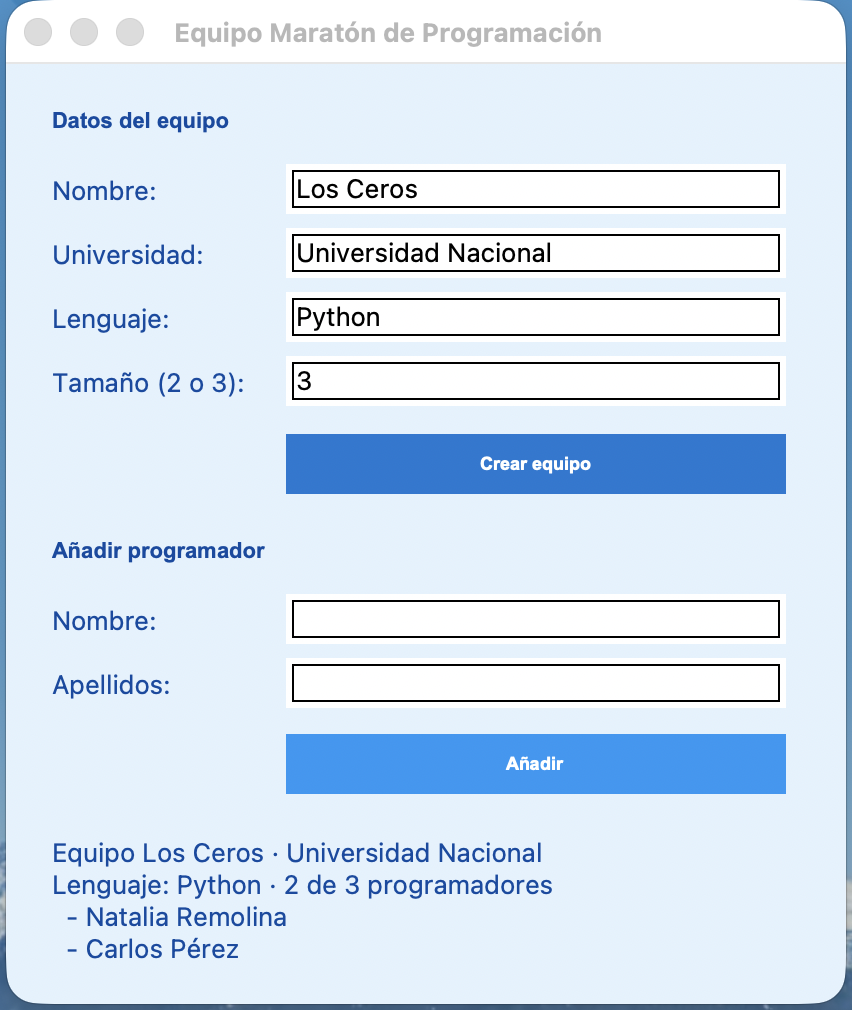
\includegraphics[width=0.46\textwidth]{equipo.png}
    \caption{Equipo creado, con dos de sus tres programadores añadidos.}
\end{figure}

\subsection{Código fuente}
\begin{lstlisting}
import tkinter as tk
from tkinter import messagebox, ttk

# ==========================================
# CLASES LÓGICAS (Modelo)
# ==========================================
class Programador:
    """Integrante del equipo. Valida que su nombre y apellidos sean
    solo texto y que no lleguen a 20 caracteres."""

    LONGITUD_MAXIMA = 20

    def __init__(self, nombre, apellidos):
        self.validar_campo(nombre, "nombre")
        self.validar_campo(apellidos, "apellidos")
        self.nombre = nombre
        self.apellidos = apellidos

    def validar_campo(self, texto, etiqueta):
        """Lanza una excepción si el campo tiene dígitos o es muy largo."""
        if not texto:
            raise ValueError(f"El campo {etiqueta} no puede estar vacío")
        for caracter in texto:
            if caracter.isdigit():
                raise ValueError(f"El campo {etiqueta} solo admite texto")
        if len(texto) >= self.LONGITUD_MAXIMA:
            raise ValueError(f"El campo {etiqueta} no puede tener "
                             f"{self.LONGITUD_MAXIMA} caracteres o más")

class EquipoMaratonProgramacion:
    """Equipo que participa en la maratón. Admite mínimo dos
    programadores y máximo tres."""

    MINIMO = 2
    MAXIMO = 3

    def __init__(self, nombre, universidad, lenguaje, tamano):
        if tamano < self.MINIMO or tamano > self.MAXIMO:
            raise ValueError(f"El equipo debe tener entre {self.MINIMO} "
                             f"y {self.MAXIMO} programadores")
        self.nombre = nombre
        self.universidad = universidad
        self.lenguaje = lenguaje
        self.tamano = tamano
        self.programadores = []

    def esta_completo(self):
        """Indica si ya se alcanzó el tamaño definido para el equipo."""
        return len(self.programadores) == self.tamano

    def anadir_programador(self, programador):
        """Agrega un programador. Lanza una excepción si el equipo está lleno."""
        if self.esta_completo():
            raise ValueError("El equipo ya está completo, no admite más programadores")
        self.programadores.append(programador)

# ==========================================
# CLASE INTERFAZ GRÁFICA (Vista/Controlador)
# ==========================================
class VentanaEquipo(tk.Tk):
    """Ventana que crea el equipo y le añade sus programadores."""

    def __init__(self):
        super().__init__()

        # Paleta de colores azul
        self.color_fondo = "#e3f2fd"
        self.color_texto = "#0d47a1"

        self.title("Equipo Maratón de Programación")
        self.geometry("420x470")
        self.resizable(False, False)
        self.configure(bg=self.color_fondo)

        self.equipo = None

        self._crear_estilos()
        self._crear_componentes()
        self.eval('tk::PlaceWindow . center')

    def _crear_estilos(self):
        # Se usa ttk con el tema "clam" porque los botones tk no admiten
        # colores de fondo en macOS y quedarían ilegibles.
        estilo = ttk.Style(self)
        estilo.theme_use("clam")
        estilo.configure("Azul.TButton", background="#2196f3", foreground="white",
                         font=("Arial", 9, "bold"), borderwidth=0, focuscolor="#2196f3")
        estilo.map("Azul.TButton", background=[("active", "#1565c0")])
        estilo.configure("AzulOscuro.TButton", background="#1976d2", foreground="white",
                         font=("Arial", 9, "bold"), borderwidth=0, focuscolor="#1976d2")
        estilo.map("AzulOscuro.TButton", background=[("active", "#0d47a1")])

    def _crear_componentes(self):
        titulo_style = {"bg": self.color_fondo, "fg": self.color_texto,
                        "font": ("Arial", 11, "bold"), "anchor": "w"}
        campo_style = {"bg": self.color_fondo, "fg": self.color_texto, "anchor": "w"}

        # --- Datos del equipo ---
        tk.Label(self, text="Datos del equipo", **titulo_style).place(x=20, y=15, width=200, height=25)

        etiquetas_equipo = ["Nombre:", "Universidad:", "Lenguaje:", "Tamaño (2 o 3):"]
        self.entradas_equipo = []
        for i, texto in enumerate(etiquetas_equipo):
            tk.Label(self, text=texto, **campo_style).place(x=20, y=50 + (i * 32), width=110, height=25)
            txt_entry = tk.Entry(self, bd=1, relief="solid")
            txt_entry.place(x=140, y=50 + (i * 32), width=250, height=25)
            self.entradas_equipo.append(txt_entry)

        ttk.Button(self, text="Crear equipo", command=self.action_crear_equipo,
                   style="AzulOscuro.TButton").place(x=140, y=185, width=250, height=30)

        # --- Programadores ---
        tk.Label(self, text="Añadir programador", **titulo_style).place(x=20, y=230, width=220, height=25)

        etiquetas_programador = ["Nombre:", "Apellidos:"]
        self.entradas_programador = []
        for i, texto in enumerate(etiquetas_programador):
            tk.Label(self, text=texto, **campo_style).place(x=20, y=265 + (i * 32), width=110, height=25)
            txt_entry = tk.Entry(self, bd=1, relief="solid")
            txt_entry.place(x=140, y=265 + (i * 32), width=250, height=25)
            self.entradas_programador.append(txt_entry)

        ttk.Button(self, text="Añadir", command=self.action_anadir,
                   style="Azul.TButton").place(x=140, y=335, width=250, height=30)

        # --- Estado del equipo ---
        self.lbl_estado = tk.Label(self, text="Primero cree el equipo.",
                                   justify="left", **campo_style)
        self.lbl_estado.place(x=20, y=380, width=380, height=75)

    def action_crear_equipo(self):
        """Crea el equipo con los datos ingresados."""
        nombre, universidad, lenguaje, tamano_texto = [e.get().strip() for e in self.entradas_equipo]

        if not nombre or not universidad or not lenguaje or not tamano_texto:
            messagebox.showwarning("Datos incompletos",
                                   "Debe diligenciar los cuatro datos del equipo.")
            return

        try:
            tamano = int(tamano_texto)
        except ValueError:
            messagebox.showerror("Error", "El tamaño debe ser un número entero.")
            return

        try:
            self.equipo = EquipoMaratonProgramacion(nombre, universidad, lenguaje, tamano)
            self.mostrar_estado()
        except ValueError as excepcion:
            self.equipo = None
            messagebox.showerror("Tamaño no válido", str(excepcion))

    def action_anadir(self):
        """Añade un programador al equipo, validando sus datos."""
        if self.equipo is None:
            messagebox.showwarning("Sin equipo", "Primero debe crear el equipo.")
            return

        nombre, apellidos = [e.get().strip() for e in self.entradas_programador]

        try:
            programador = Programador(nombre, apellidos)
            self.equipo.anadir_programador(programador)
            for entrada in self.entradas_programador:
                entrada.delete(0, tk.END)
            self.mostrar_estado()
        except ValueError as excepcion:
            # Una misma excepción cubre los datos inválidos y el equipo lleno
            messagebox.showerror("No se pudo añadir", str(excepcion))

    def mostrar_estado(self):
        """Muestra los datos del equipo y la lista de sus programadores."""
        lineas = [f"Equipo {self.equipo.nombre} · {self.equipo.universidad}",
                  f"Lenguaje: {self.equipo.lenguaje} · "
                  f"{len(self.equipo.programadores)} de {self.equipo.tamano} programadores"]

        for programador in self.equipo.programadores:
            lineas.append(f"  - {programador.nombre} {programador.apellidos}")

        if self.equipo.esta_completo():
            lineas.append("El equipo está completo.")

        self.lbl_estado.config(text="\n".join(lineas))

# ==========================================
# BLOQUE PRINCIPAL
# ==========================================
if __name__ == "__main__":
    app = VentanaEquipo()
    app.mainloop()
\end{lstlisting}

\newpage
% ---------------------------------------------------------
% EJERCICIO 4.5
% ---------------------------------------------------------
\section{Ejercicio 6.8. Lectura de archivos: clase LeerArchivo}

\subsection{Enunciado}
Se tiene un archivo de texto denominado \texttt{prueba.txt} en una cierta localización del
sistema de archivos. Se requiere desarrollar un programa que lea dicho archivo utilizando un
flujo de datos y muestre su contenido en pantalla.

\medskip
\noindent La solución permite además escoger cualquier otro archivo de texto del computador, y
captura la excepción de entrada y salida que se produce cuando el archivo no existe o no se
puede leer. El archivo se cierra siempre, dentro de un bloque \texttt{finally}.

\noindent \textbf{Enlace al repositorio en GitHub:} \\
\url{https://github.com/NatoRemolina/UNAL-Programacion-Orientada-a-Objetos/blob/main/actividad-04/ejercicio5.py}

\subsection{Diagrama de clases}
\clasebox{LeerArchivo}
{%
- ruta \\
}
{%
+ leer() \\
}

\clasebox{VentanaLector}
{%
- lbl\_ruta \\
- txt\_contenido \\
}
{%
+ \_crear\_componentes() \\
+ action\_abrir() \\
+ action\_leer\_prueba() \\
+ mostrar\_archivo() \\
+ escribir() \\
}

\noindent \textbf{Relaciones:}
\begin{itemize}
    \item \texttt{VentanaLector} hereda de \texttt{tk.Tk}.
    \item \texttt{VentanaLector} usa a \texttt{LeerArchivo} (dependencia): le entrega una ruta y recibe el contenido, o captura la excepción de lectura.
\end{itemize}

\subsection{Casos de uso}
\begin{table}[H]
\centering
\begin{tabularx}{\textwidth}{@{}l X@{}}
\toprule
\textbf{Caso de uso} & CU-01: Leer el archivo de prueba \\
\midrule
\textbf{Actor} & Usuario \\
\textbf{Precondición} & La ventana está abierta. \\
\textbf{Flujo principal} & 1. El usuario presiona el botón \textit{Leer prueba.txt}. \newline 2. El sistema abre el archivo que acompaña al ejercicio. \newline 3. El sistema muestra su contenido y el nombre del archivo. \newline 4. El sistema cierra el archivo. \\
\textbf{Flujo alterno A} & En el paso 2, si el archivo no existe o no se puede leer, el sistema muestra la excepción \textit{``No se encontró el archivo''}. El caso de uso termina. \\
\textbf{Postcondición} & El contenido del archivo queda visible en la ventana. \\
\bottomrule
\end{tabularx}
\end{table}

\begin{table}[H]
\centering
\begin{tabularx}{\textwidth}{@{}l X@{}}
\toprule
\textbf{Caso de uso} & CU-02: Abrir otro archivo \\
\midrule
\textbf{Actor} & Usuario \\
\textbf{Precondición} & La ventana está abierta. \\
\textbf{Flujo principal} & 1. El usuario presiona el botón \textit{Abrir archivo}. \newline 2. El sistema muestra el explorador de archivos del computador. \newline 3. El usuario selecciona un archivo de texto. \newline 4. El sistema lee el archivo y muestra su contenido. \\
\textbf{Flujo alterno A} & En el paso 3, si el usuario cancela, no se hace nada y el caso de uso termina. \\
\textbf{Postcondición} & El contenido del archivo escogido queda visible en la ventana. \\
\bottomrule
\end{tabularx}
\end{table}

\subsection{Interfaz de usuario}
\begin{figure}[H]
    \centering
    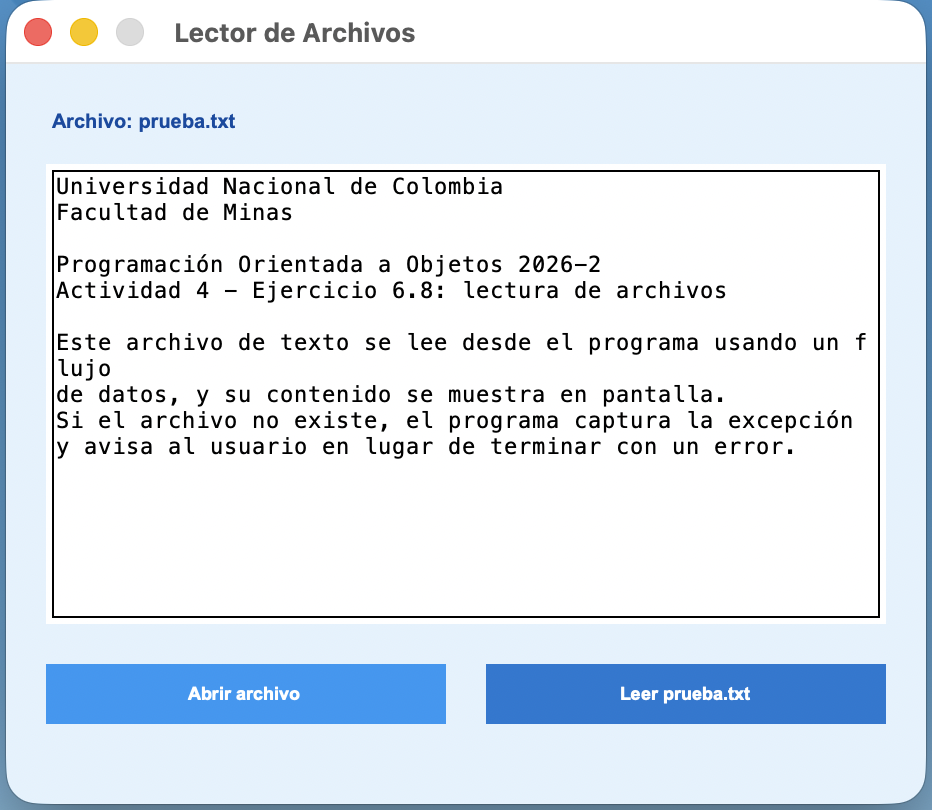
\includegraphics[width=0.58\textwidth]{archivo.png}
    \caption{Contenido del archivo prueba.txt mostrado en la ventana.}
\end{figure}

\subsection{Código fuente}
\begin{lstlisting}
import tkinter as tk
from tkinter import filedialog, messagebox, ttk
import os

# ==========================================
# CLASE LÓGICA (Modelo)
# ==========================================
class LeerArchivo:
    """Lee un archivo de texto y entrega su contenido.
    Gestiona los errores de entrada y salida."""

    def __init__(self, ruta):
        self.ruta = ruta

    def leer(self):
        """Retorna el contenido del archivo.
        Lanza una excepción si no existe o no se puede leer."""
        archivo = None
        try:
            archivo = open(self.ruta, "r", encoding="utf-8")
            return archivo.read()
        except FileNotFoundError:
            raise IOError(f"No se encontró el archivo: {self.ruta}")
        except OSError:
            raise IOError(f"No se pudo leer el archivo: {self.ruta}")
        finally:
            # El archivo se cierra siempre, ocurra o no una excepción
            if archivo is not None:
                archivo.close()

# ==========================================
# CLASE INTERFAZ GRÁFICA (Vista/Controlador)
# ==========================================
class VentanaLector(tk.Tk):
    """Ventana que permite escoger un archivo de texto y ver su contenido."""

    ARCHIVO_POR_DEFECTO = "prueba.txt"

    def __init__(self):
        super().__init__()

        # Paleta de colores azul
        self.color_fondo = "#e3f2fd"
        self.color_texto = "#0d47a1"

        self.title("Lector de Archivos")
        self.geometry("460x370")
        self.resizable(False, False)
        self.configure(bg=self.color_fondo)

        self._crear_componentes()
        self.eval('tk::PlaceWindow . center')

    def _crear_componentes(self):
        self.lbl_ruta = tk.Label(self, text="Ningún archivo abierto",
                                 bg=self.color_fondo, fg=self.color_texto,
                                 anchor="w", font=("Arial", 10, "bold"))
        self.lbl_ruta.place(x=20, y=15, width=420, height=25)

        # Área donde se muestra el contenido del archivo
        self.txt_contenido = tk.Text(self, bd=1, relief="solid")
        self.txt_contenido.place(x=20, y=50, width=420, height=230)
        self.txt_contenido.config(state="disabled")

        # Botones con estilo azul.
        # Se usa ttk con el tema "clam" porque los botones tk no admiten
        # colores de fondo en macOS y quedarían ilegibles.
        estilo = ttk.Style(self)
        estilo.theme_use("clam")
        estilo.configure("Abrir.TButton", background="#2196f3", foreground="white",
                         font=("Arial", 9, "bold"), borderwidth=0, focuscolor="#2196f3")
        estilo.map("Abrir.TButton", background=[("active", "#1565c0")])
        estilo.configure("Prueba.TButton", background="#1976d2", foreground="white",
                         font=("Arial", 9, "bold"), borderwidth=0, focuscolor="#1976d2")
        estilo.map("Prueba.TButton", background=[("active", "#0d47a1")])

        ttk.Button(self, text="Abrir archivo", command=self.action_abrir,
                   style="Abrir.TButton").place(x=20, y=300, width=200, height=30)
        ttk.Button(self, text="Leer prueba.txt", command=self.action_leer_prueba,
                   style="Prueba.TButton").place(x=240, y=300, width=200, height=30)

    def action_abrir(self):
        """Permite escoger un archivo de texto del sistema de archivos."""
        ruta = filedialog.askopenfilename(
            title="Seleccione un archivo de texto",
            filetypes=[("Archivos de texto", "*.txt"), ("Todos los archivos", "*.*")])
        if ruta:
            self.mostrar_archivo(ruta)

    def action_leer_prueba(self):
        """Lee el archivo prueba.txt que acompaña al ejercicio."""
        carpeta = os.path.dirname(os.path.abspath(__file__))
        self.mostrar_archivo(os.path.join(carpeta, self.ARCHIVO_POR_DEFECTO))

    def mostrar_archivo(self, ruta):
        """Muestra el contenido del archivo o la excepción generada."""
        lector = LeerArchivo(ruta)
        try:
            contenido = lector.leer()
        except IOError as excepcion:
            self.lbl_ruta.config(text="Ningún archivo abierto")
            self.escribir("")
            messagebox.showerror("Error de lectura", str(excepcion))
            return

        self.lbl_ruta.config(text="Archivo: " + os.path.basename(ruta))
        self.escribir(contenido)

    def escribir(self, texto):
        """Vuelca un texto en el área de contenido."""
        self.txt_contenido.config(state="normal")
        self.txt_contenido.delete("1.0", tk.END)
        self.txt_contenido.insert(tk.END, texto)
        self.txt_contenido.config(state="disabled")

# ==========================================
# BLOQUE PRINCIPAL
# ==========================================
if __name__ == "__main__":
    app = VentanaLector()
    app.mainloop()
\end{lstlisting}

\end{document}
